%<dscrpt>Chemins et nombres de Catalan.</dscrpt>
Pour tout le problème, $a$ et $b$ désignent des entiers naturels tels que $a < b$. 
Dans un plan muni d'un repère orthonormé $(O,(\overrightarrow i , \overrightarrow j))$ dont les fonctions coordonnées sont notées $x$ et $y$, on fixe certaines définitions et notations.
\begin{itemize}
 \item Un point $M$ est \emph{sur la diagonale} si et seulement si $x(M) = y(M)$.
 \item Un point $M$ est \emph{au dessous de la diagonale} si et seulement si $y(M) \leq x(M)$.
 \item Un point $M$ est \emph{strictement au dessous de la diagonale} si et seulement si $y(M) < x(M)$.
 \item On appelle \emph{chemin} une famille de points à coordonnées entières 
\begin{displaymath}
 (M_0,M_1,\cdots M_p) \text{ tq } \forall k\in \llbracket 0, p-1 \rrbracket,\; 
\overrightarrow{M_kM_{k+1}}\in \{\overrightarrow i , \overrightarrow j\}
\end{displaymath}
On dit que les $M_k$ sont les points du chemin, que ce chemin est de longueur $p$ et qu'il va de $M_0$ à $M_p$ (extrémités du chemin).
 \item On désigne par $\mathcal{P}_{a,b}$ l'ensemble des chemins allant du point de coordonnées $(a,a)$ au point de coordonnées  $(b,b)$.
 \item On désigne par $\mathcal{C}_{a,b}$ l'ensemble des chemins appartenant à $\mathcal{P}_{a,b}$ et dont tous les points sont au dessous de la diagonale.
 \item On désigne par $\mathcal{C}'_{a,b}$ l'ensemble des chemins appartenant à $\mathcal{P}_{a,b}$ et dont tous les points (sauf les extrémités) sont strictement au dessous de la diagonale.
 \item Si $\Gamma = (M_0,M_1,\cdots M_p)\in \mathcal{C}_{a,b}$, on note $m(\Gamma)$ le plus petit des $x(M_k)>0$ tels que $M_k$ soit sur la diagonale.
 \item Pour $n\in \N^*$, on note $c_n$ le nombre d'éléments de $\mathcal{C}_{0,n}$. On convient que $c_0=1$.
\end{itemize}
La figure \ref{fig: Enbcat_1} montre le dessin obtenu en reliant les points d'un chemin $\Gamma \in \mathcal{C}_{0,5}$ par des segments. Que vaut $m(\Gamma)$ sur cet exemple?
\begin{figure}[h!t]
 \centering
 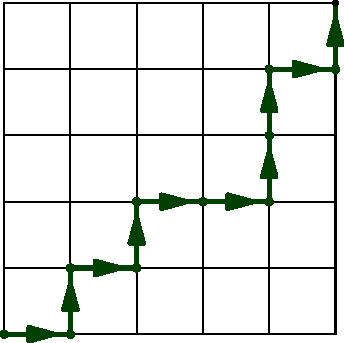
\includegraphics{./Enbcat_1.pdf}
 % Enbcat_1.pdf: 0x0 pixel, 0dpi, 0.00x0.00 cm, bb=
 \caption{Chemin appartenant à $\mathcal{C}_{0,5}$}
 \label{fig: Enbcat_1}
\end{figure}
  
\begin{enumerate}
 \item Soit $n\in \N^*$.
\begin{enumerate} 
 \item Quelle est la longueur d'un chemin appartenant à $\mathcal{P}_{0,n}$ ?
 \item Calculer le nombre d'éléments de $\mathcal{P}_{0,n}$ en le mettant en bijection avec un ensemble usuel.
\end{enumerate}
\item 
\begin{enumerate}
 \item Préciser $c_1$ et $c_2$.
 \item Exprimer le nombre d'éléments de $\mathcal{C}_{a,b}$ à l'aide d'un $c_k$ pour un entier $k$ à préciser.
 \item Soit $m\in \N^*$, exprimer le nombre d'éléments de $\mathcal{C}'_{0,m}$ à l'aide d'un $c_k$ pour un entier $k$ à préciser.
 \item Montrer que
\begin{displaymath}
 \forall n\in \N^*,\; c_n =\sum_{m=1}^{n}c_{m-1}c_{n-m} 
\end{displaymath}
En déduire que
\begin{displaymath}
 \forall n\in \N,\; c_{n+1} =\sum_{k=0}^{n}c_{k}c_{n-k} 
\end{displaymath}
\end{enumerate}
\item Les nombres $c_n$ sont appelés les \emph{nombres de Catalan}, ils interviennent dans diverses questions de dénombrement. On se propose de démontrer par récurrence que
\begin{displaymath}
 c_n = \frac{\binom{2n}{n}}{n+1}
\end{displaymath}
Dans cette question, $n$ est un naturel quelconque, notons
\begin{displaymath}
 a_n= \frac{\binom{2n}{n}}{n+1}
,\hspace{0.5cm} S_{n} =\sum_{k=0}^{n}a_{k}a_{n-k}
,\hspace{0.5cm} T_{n} =\sum_{k=0}^{n}ka_{k}a_{n-k}
\end{displaymath}
en convenant que $a_0=1$. 
\begin{enumerate}
 \item Montrer $2T_n = n S_n$. En déduire $T_{n+1}+S_{n+1} = \frac{n+3}{2}S_{n+1}$.
 \item Montrer $(k+2)a_{k+1} = 2(2k+1)a_k$. En déduire $ T_{n+1}+S_{n+1} = a_{n+1} + 4T_n +2S_n $.
 \item Montrer que $S_n=a_{n+1}$ entraine $S_{n+1}=a_{n+2}$ et conclure.
\end{enumerate}

\end{enumerate}
